% This section will focus on the algorithm implementations, ROS2 data flow, metrics, and experiment design.
% It will detail the localization algorithms for dead reckoning \cite{ros2_control_mobile_robot_kinematics}, extended kalman filter (EKF) \cite{leonard1991mobile}, and particle filter (PF) \cite{doucet2000sequential}.
% It will describe scan matching, including the iterative closest point (ICP) algorithm \cite{besl1992method}, as well as, details on the SVD-based rigid transformation \cite{arun1987least}.
% Furthermore, this section will detail the design of Monte Carlo Localization (MCL) algorithm for the PF \cite{fox1999monte}.
% If time permits, this section will describe a hybrid algorithm in which the PF detects potential kidnapping events and supports EKF recovery by providing a pose estimate and an uncertainty estimate derived from the particle distribution.

% The study approach section will continue with ROS2 node graph and data flow focusing on the inputs and outputs for the localization algorithms.
% It will detail where data is being produced, where noise is being injected, and the plans for storing the data for analysis.
% Next, this section will detail the metrics that will be collected at each time step including position error, heading error, and compute cost.
% Finally, this section will detail the experimental design for test cases including a uniform prior, mid-run kidnapping, the sensitivity analyses on varying particle count, injected odometry noise, and injected LiDAR noise.

\section{Study Approach}\label{Study-Approach}
This section begins by outlining the model that the three algorithms share including the mobile platform and its sensors, the kinematic model and its Jacobians, the odometry noise model, and the map representations.
Then it describes the algorithms and their implementation specifics.
At the end, this section describes the mechanisms for kidnapping in the Gazebo environment and the metrics to be collected in the experiments presented in section \ref{sec:Results}.

\subsection{System Model}
A high level overview of the ROS2 system used in this study is illustrated in Figure \ref{fig:full_system_diagram}.
The algorithms under test represent the \texttt{AgentLocalizer} box in gold.
It receives sensor data from Gazebo plugins, described below.
Additionally, the \texttt{AgentLocalizer} subscribes to a map representation generated from an octomap\_server node.
The \texttt{AgentLocalizer} publishes its pose to a local motion planner and a position controller.
The position controller then sends commands to a Gazebo DiffDrive \cite{gazebo_diff_drive} plugin which sends joint velocities to the simulated robot's wheels.

\begin{figure}[!htbp]
    \centering
    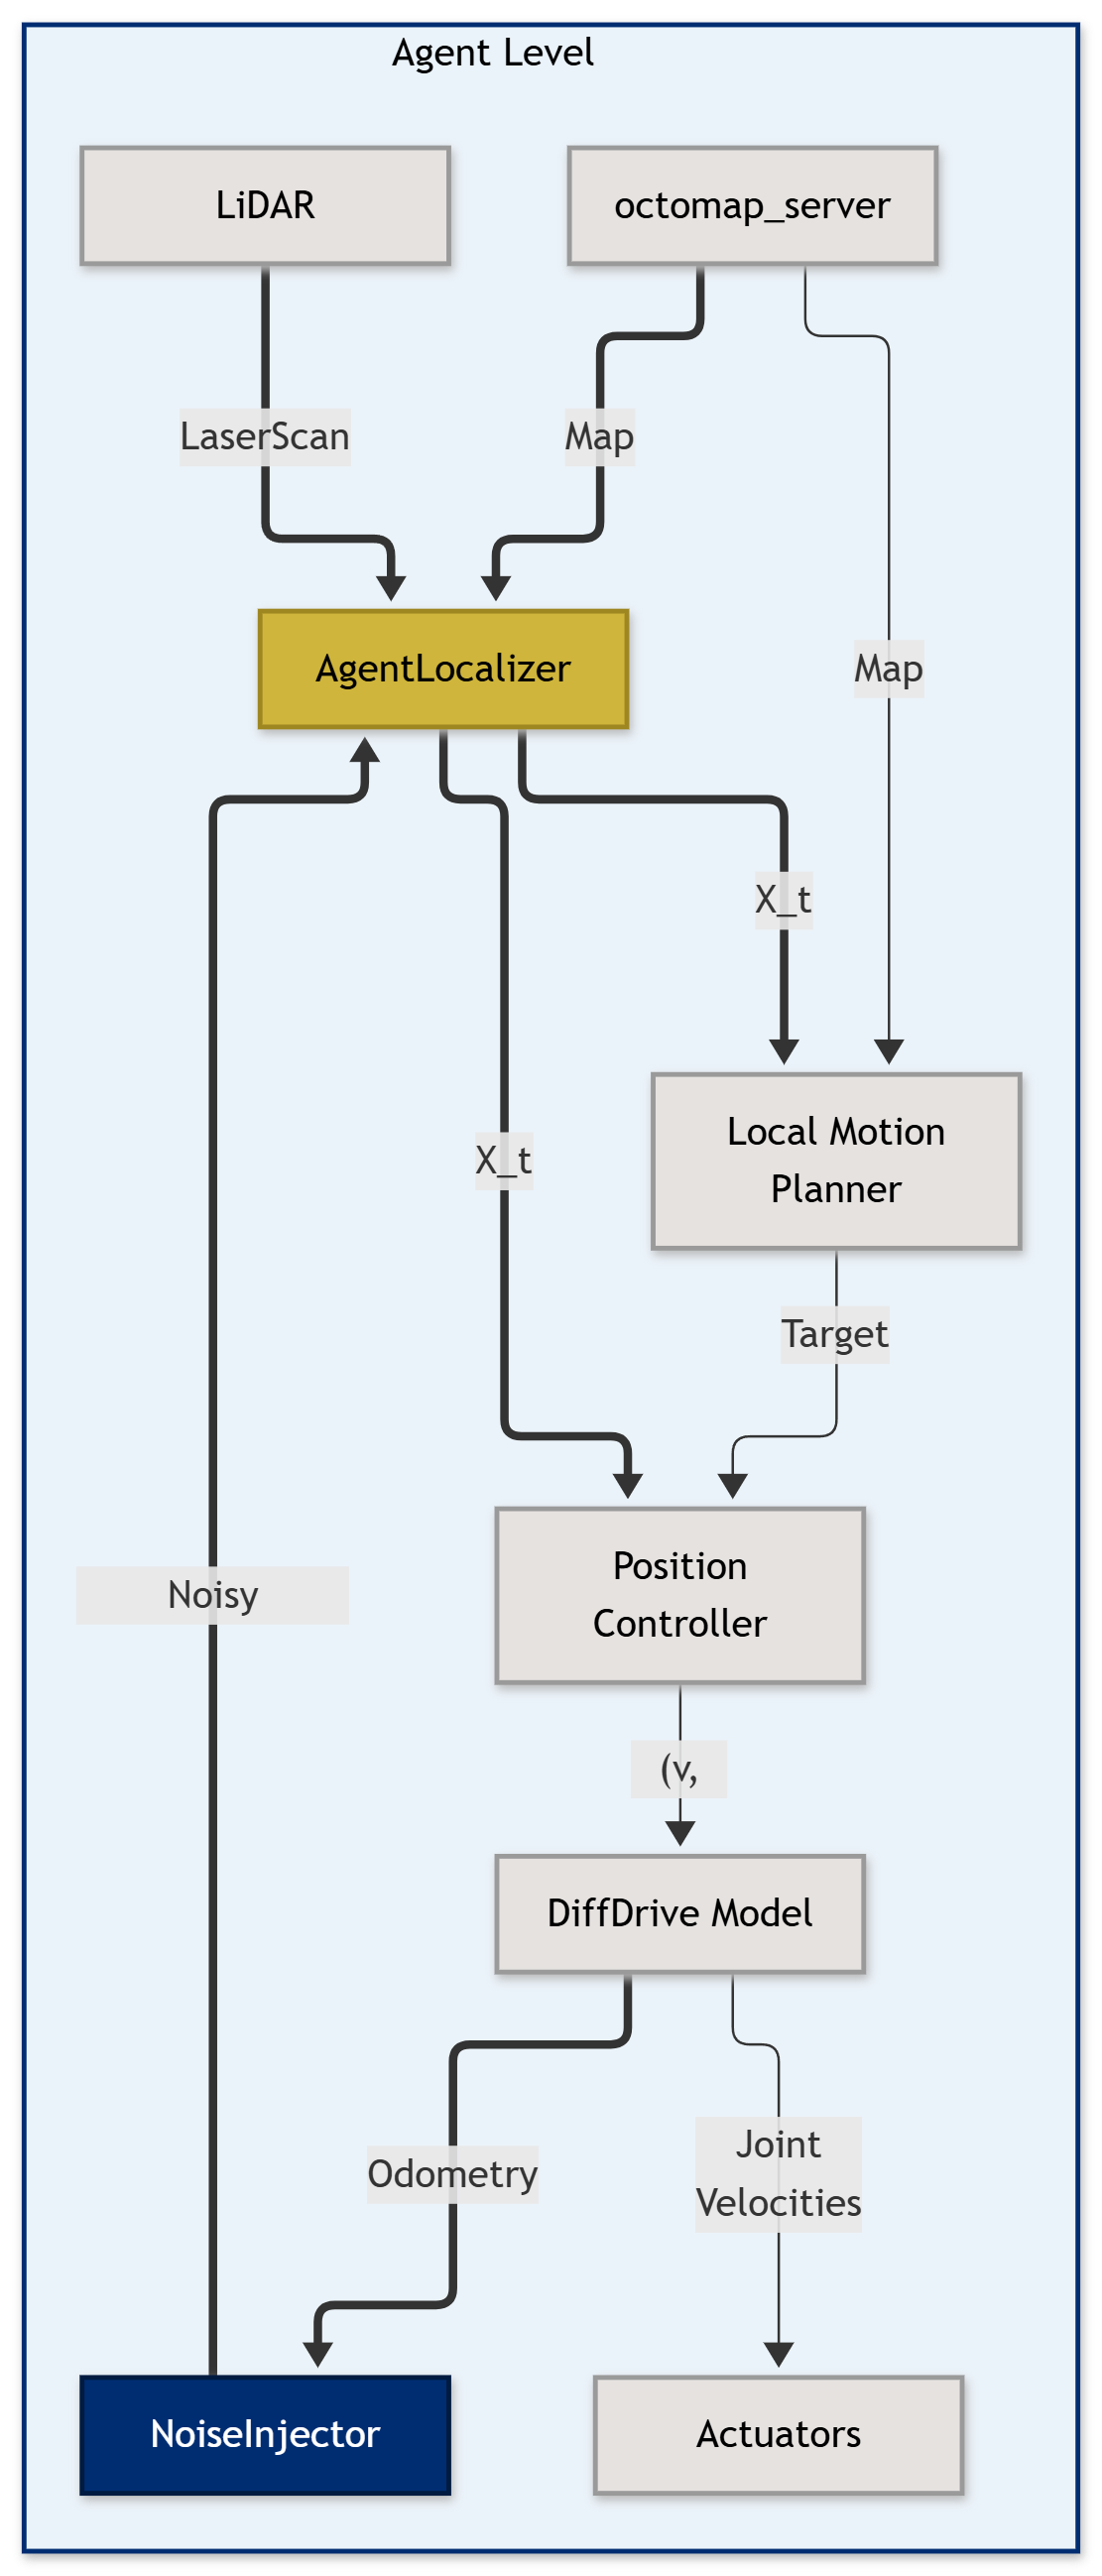
\includegraphics[width=\textwidth]{figures/full_system_diagram.png}
    \caption{Full ROS2 system diagram}
    \label{fig:full_system_diagram}
\end{figure}

The Local Motion Planner and Position Controller nodes are outside of the scope of this work.
In the experiments presented here, the local motion planner uses an RRT* algorithm \cite{karaman2011sampling}.
Both the Local Motion Planner and Position Controller nodes monitor the robot's true position through Gazebo's internal transform tree.
This is done to isolate the localization algorithm's performance without adding complexity.
In a real world application where there is no access to a ground truth transform, these localization algorithms would take the place of the transform tree lookup.

\subsubsection{Platform \& Sensors}
The robot models used in Gazebo and ROS2 are defined using Unified Robot Description Format (URDF).
This study will use the mobile manipulator model illustrated in Figure \ref{fig:devol_robot_model}.
It consists of a Husky A200 differential drive mobile platform with a mounted $270^\circ$ 2-D LiDAR and a manipulator.
The manipulator comprises a Universal Robots UR5e collaborative robot arm and a Robotiq 2F-85 end effector.
Plugins for Differential Drive, odometry, wheel slip, and LiDAR from Gazebo were leveraged to add model the sensors and actuators in the simulated factory.

\begin{figure}[!htbp]
    \centering
    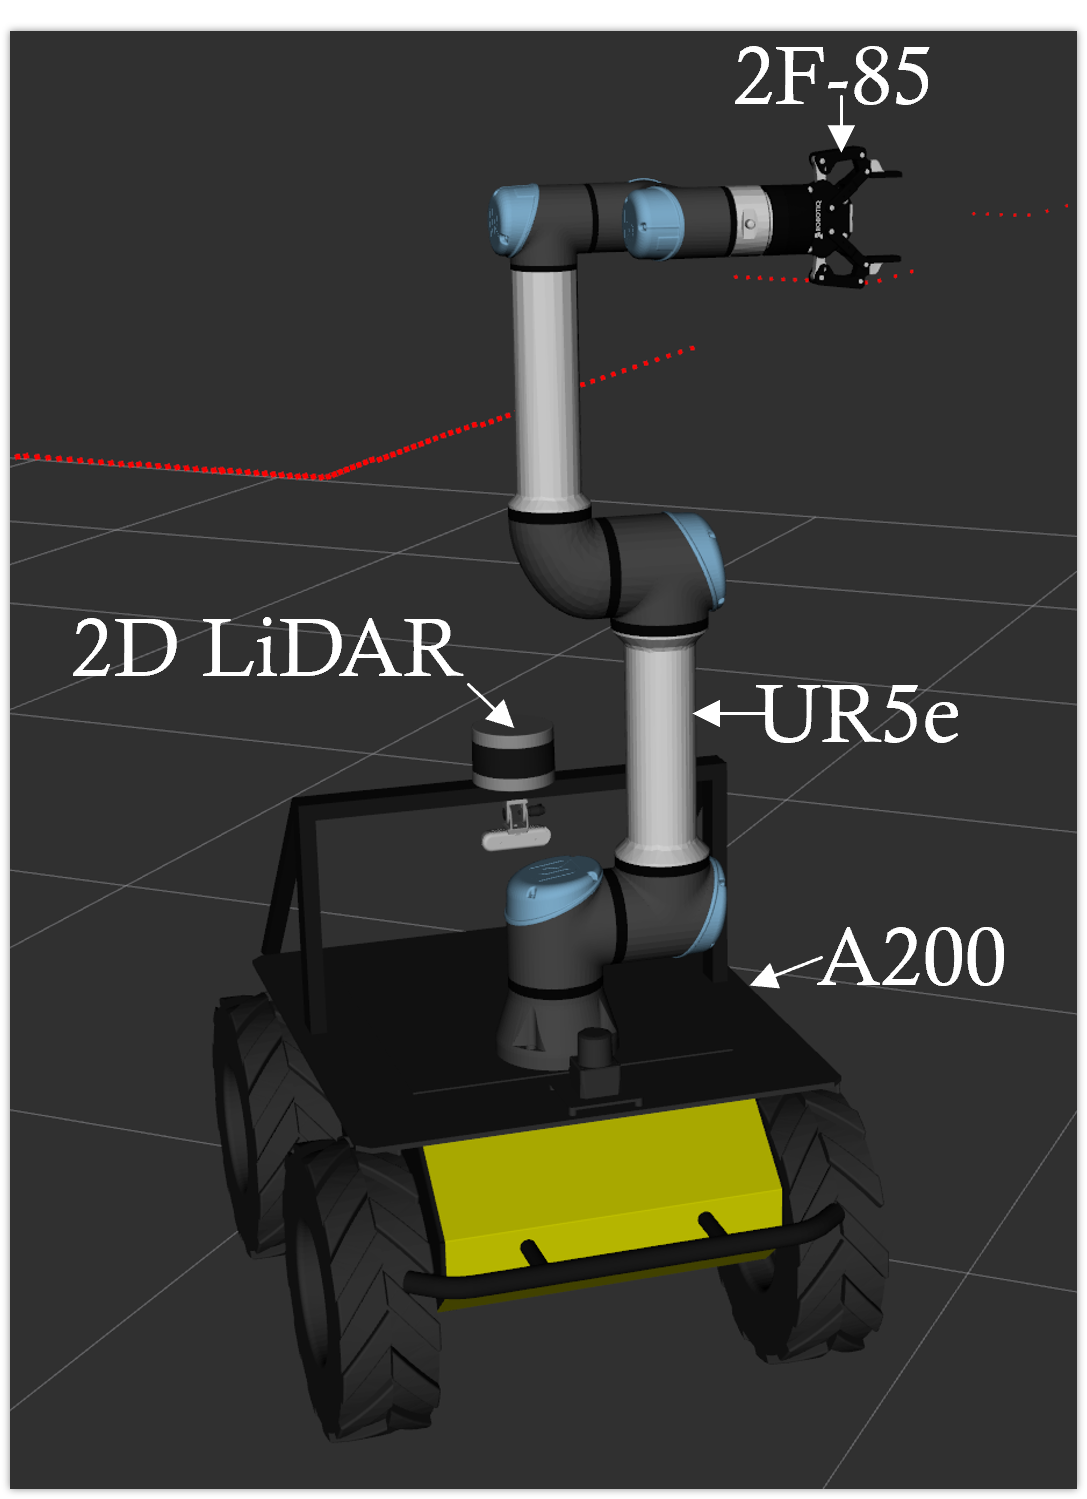
\includegraphics[width=.25\textwidth]{figures/devol_robot_model.png}
    \caption{Test robot model.}
    \label{fig:devol_robot_model}
\end{figure}

\textbf{Odometry:} The \texttt{DiffDrive} plugin \cite{gazebo_diff_drive} is used to both publish \texttt{nav\_msgs/Odometry} messages and receive velocity commands in the form of $u_t=\begin{bmatrix} v_t \\ \omega_t \end{bmatrix}$. 
The \texttt{WheelSlip} \cite{gazebo_wheel_slip} plugin is used to create uncertainty in the odometry to match real world applications.
The robot's odometry publishes at 30 Hz.
Additionally, \texttt{OdometryPublisher} \cite{gazebo_odom} is used to publish the ground truth odometry and transform for results comparison.

\textbf{LiDAR:} The Lidar plugin \cite{gazebo_lidar} is used to generate \texttt{sensor\_msgs/LaserScan} messages.
The beam spans $[\phi_{min},\phi_{max}]=[-2.356,2.356]$.
The transform from the base of the model to the LiDAR frame is static and was calculated with the tf2\_tools as $t_L=[0.32825,0.0,0.0]^T$.
The LiDAR scans are preprocessed by the localization algorithms using the same method.
Rays that are outside of nominal range, as defined by the \texttt{sensor\_msgs/LaserScan} message, are thrown out.

\subsubsection{Unicycle Kinematics}
Since the odometry is produced in the form of $u_t=\begin{bmatrix} v_t \\ \omega_t \end{bmatrix}$, the kinematic model can be reduced to a Unicycle Kinematic model.

\textbf{Forward Kinematics:} The ros2\_controllers page on wheeled kinematics \cite{ros2_control_mobile_robot_kinematics} provides the forward kinematics of the unicycle for continuous time shown in Equation \ref{eq:continuous_unicycle_kinematics}.

\begin{equation}\label{eq:continuous_unicycle_kinematics}
    \begin{bmatrix} \dot{x} \\ \dot{y} \\ \dot{\theta} \end{bmatrix} = \begin{bmatrix}
        v_{b,x}\cos(\theta) \\ v_{b,x}\sin(\theta) \\ \omega_{b,z}
    \end{bmatrix}
\end{equation}

This can be extended to the discrete case as shown in Equation \ref{eq:discrete_unicycle_kinematics}:

\begin{equation}\label{eq:discrete_unicycle_kinematics}
    f(\textbf{x},\textbf{u},\Delta t) = \bar{\textbf{x}}_t = \begin{bmatrix}
        x + v \cos(\theta) \Delta t \\ y + v \sin(\theta) \Delta t \\ \theta + \omega \Delta t
    \end{bmatrix}
\end{equation}

\textbf{State Jacobian:} The state Jacobian $\textbf{A}_t$ is calculated by finding the partial derivatives of equation \ref{eq:discrete_unicycle_kinematics} with respect to $\textbf{x}$.

\begin{equation}\label{eq:state_jacobian_unicycle}
    \textbf{A}_t = \frac{\partial \textbf{f}}{\partial \textbf{x}} = 
    \begin{bmatrix} 
        1 & 0 & -v \sin(\theta) \Delta t \\
        0 & 1 &  v \cos(\theta) \Delta t \\
        0 & 0 & 1
    \end{bmatrix}
\end{equation}

\textbf{Control Jacobian:} The control Jacobian $\textbf{G}_t$ is calculated by finding the partial derivatives of equation \ref{eq:discrete_unicycle_kinematics} with respect to $\textbf{u}$.

\begin{equation}\label{eq:control_jacobian_unicycle}
    \textbf{G}_t = \frac{\partial \textbf{f}}{\partial \textbf{u}} = 
    \begin{bmatrix} 
        \cos(\theta) \Delta t & 0  \\
        \sin(\theta) \Delta t & 0  \\
        0 & \Delta t
    \end{bmatrix}
\end{equation}

\subsubsection{Odometry Noise Model}
Chapter 5 of \textit{Probabilistic Robotics} by Thurn \cite{thrun2005probabilistic} provides algorithms for injecting noise into our odometry sensors.
The book argues that command states or measured sensor are subject to noise and that noise can be modeled by a zero-centered random variable with finite variance as Equation \ref{eq:motion-noise}.

\begin{equation}\label{eq:motion-noise}
    \binom{\hat{v}}{\hat{\omega}} = \binom{v}{\omega} + \binom{\sigma_{\alpha_1 \left\lvert v \right\rvert + \alpha_2 \left\lvert \omega \right\rvert}}{\sigma_{\alpha_3 \left\lvert v \right\rvert + \alpha_4 \left\lvert \omega \right\rvert}}
\end{equation}

All three algorithms in this study, leverage this concept to model the uncertainty of the odometry.
Where $\alpha_1=0.10$ represents the translational noise caused by translation.
$\alpha_2=0.01$ represents the translational noise caused by rotation.
$\alpha_3=0.01$ represents the rotational noise caused by translation.
And $\alpha_4=0.20$ represents the rotational noise caused by rotation.
These values are used to create noise proportional to the odometry control signal $u_t$ as shown in Equations \ref{eq:v-noise} and \ref{eq:omega-noise}.

\begin{equation}\label{eq:v-noise}
\sigma_v = \alpha_1 |v_t| + \alpha_2 |\omega_t|
\end{equation}
\begin{equation}\label{eq:omega-noise}
\sigma_\omega = \alpha_3 |v_t| + \alpha_4 |\omega_t|
\end{equation}

\subsubsection{Map}
The open source \texttt{octomap\_server} \cite{hornung2013octomap} is used to generate the static map.
A Point Cloud Data (PCD) file was generated of the gazebo world using the open-source \texttt{sdf2map} package \cite{sdf2map}.
The static PCD file is provided to the \texttt{octomap\_server} at runtime which then publishes an OctoGrid with $0.05m$ resolution and an OccupancyGrid which is a 2-D projection of the OctoGrid.
The bottom $0.45m$ of the point cloud is removed before applying the projection to keep the factory floor from occluding the free space.


\subsection{Dead Reckoning}\label{subsec:Dead-Reckoning}
Dead Reckoning is simplest algorithm under test.
It implements only the prediction step of the Bayes filter shown in equation \ref{eq:bayes_prediction}.
A full diagram of the implemented dead reckoning algorithm is shown in Figure \ref{fig:dead_reckoning}.
The prediction step is implemented as a callback method when the Dead Reckoning node receives a \texttt{nav\_msgs/Odometry} message.

\begin{figure}[!htbp]
    \centering
    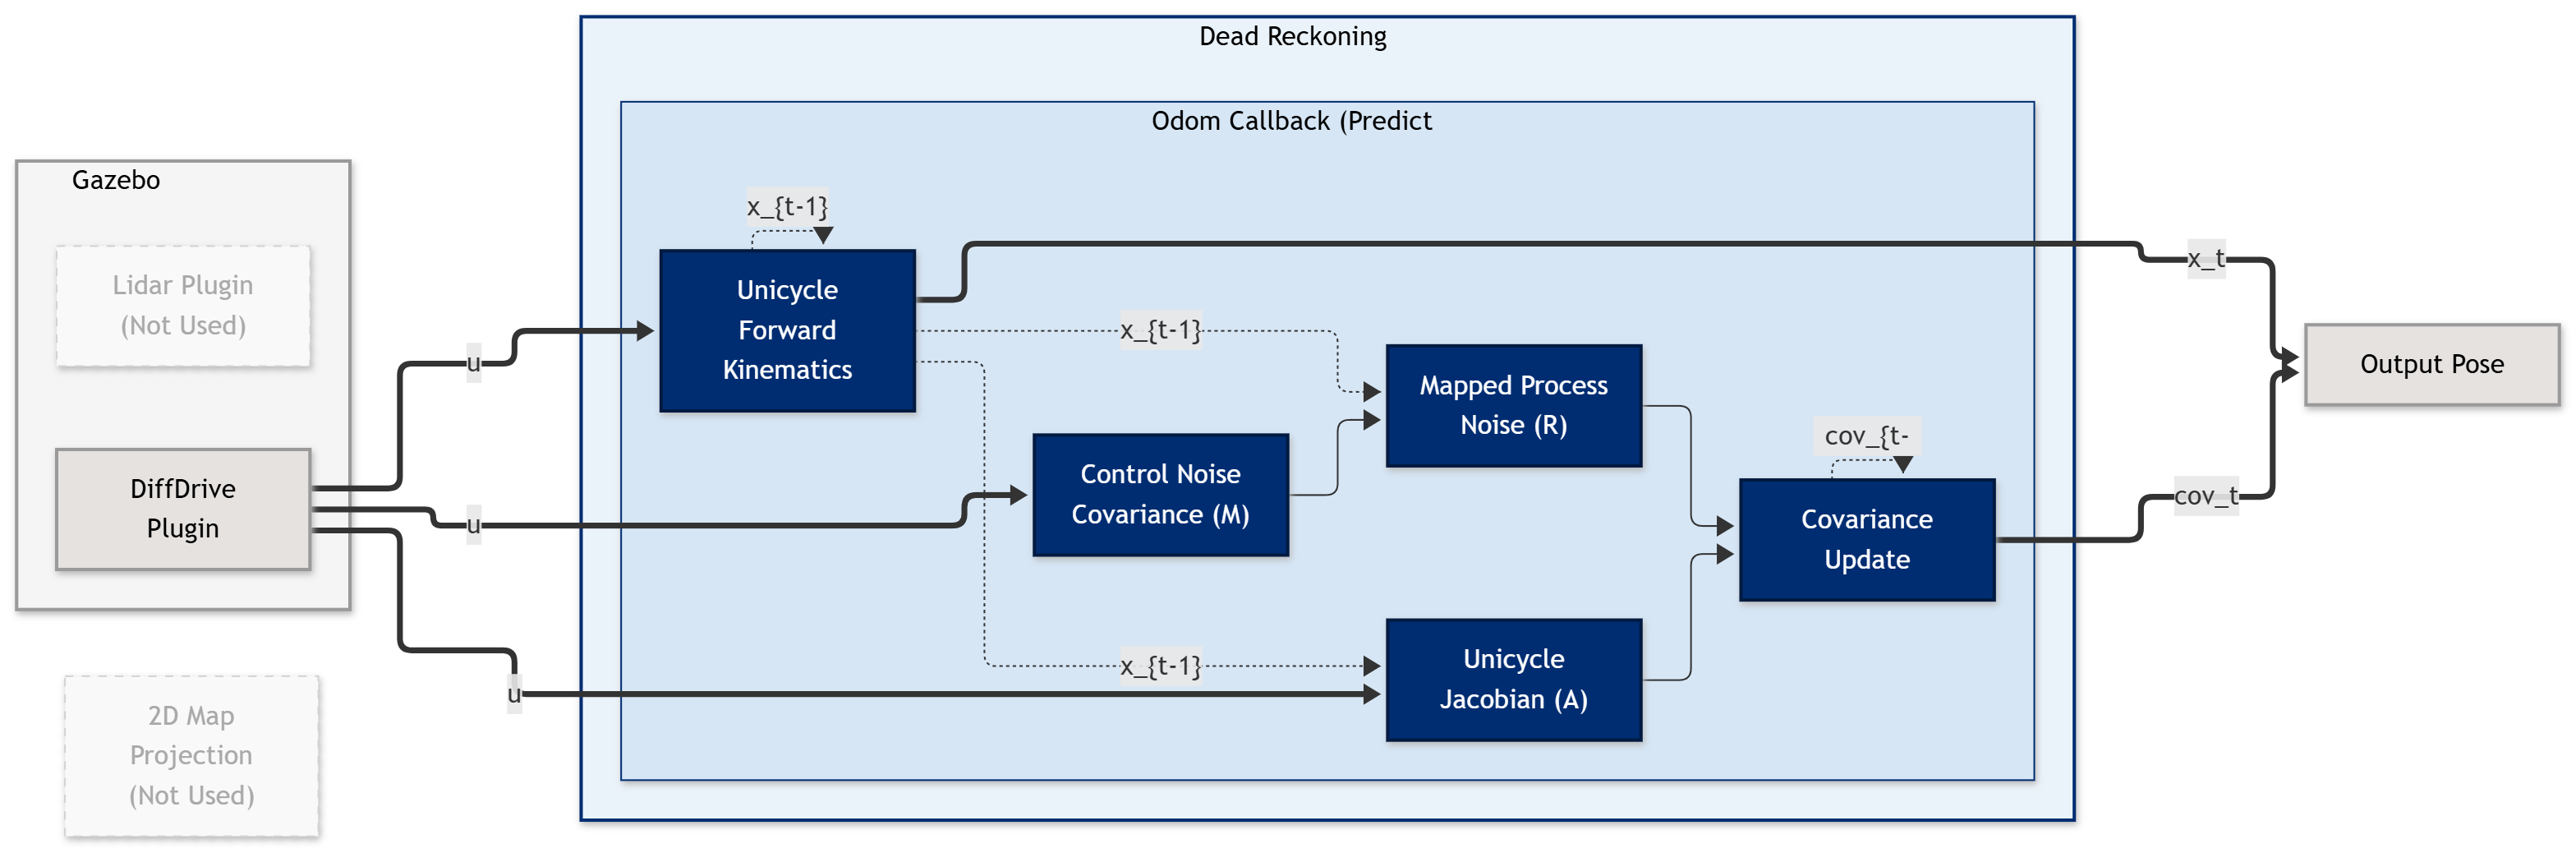
\includegraphics[width=\textwidth]{figures/dead_reckoning.png}
    \caption{Dead Reckoning Algorithm}
    \label{fig:dead_reckoning}
\end{figure}

\subsubsection{Prediction}\label{subsec:Dead-Reckoning:Prediction}
The algorithm begins by performing the forward kinematics described in Equation \ref{eq:discrete_unicycle_kinematics} to create a prediction of $\bar{\textbf{x}_t}$.
The previous state $\textbf{x}_{t-1}$ and raw Odometry message $\textbf{u}_{t}$ are used to calculate the state Jacobian $\textbf{A}_t$ shown in equation \ref{eq:state_jacobian_unicycle}.
The control noise covariance matrix $M_t$ can be calculated from the noises calculated in Equations \ref{eq:v-noise} and \ref{eq:omega-noise}:

\begin{equation} \label{eq:control_noise_covariance}
    M_t = \begin{bmatrix}
        \sigma_v^2 & 0 \\
        0 & \omega_v^2
    \end{bmatrix}
\end{equation}

The mapped process noise $R_t$ is then found using the control Jacobian as shown in Equation \ref{eq:mapped_process_noise}

\begin{equation} \label{eq:mapped_process_noise}
    R_t = G_t M_t G_t^T \Delta t
\end{equation}

Next, the covariance is updated as shown in Equation \ref{eq:dr_cov_update}.

\begin{equation} \label{eq:dr_cov_update}
    \bar{\Sigma}_t = A_t \Sigma_{t-1} A_t^T + R
\end{equation}

At the end of the predict step, the predicted values $\bar{\textbf{x}_t}$ and $\bar{\Sigma_t}$ are published as a \texttt{PoseWithCovarianceStamped} message.
The implementation of the Dead Reckoning node and algorithm can be found in Appendix \ref{subsec:DR implementation}.


\subsection{Extended Kalman Filter (EKF)}\label{subsec:EKF}
The EKF combines the Dead Reckoning prediction step implementation with an implementation of the measurement update step from Equation \ref{eq:bayes_measurement_update}.
This study's EKF uses a 2D Iterative Closest Point (ICP) scan matching algorithm to produce 

The EKF fuses the Dead Reckoning prediction with the ICP measurement update. 
Because the system is non-linear, the EKF linearizes the measurement models using Jacobians \cite{thrun2005probabilistic}.
An illustration of the EKF node is shown in Figure \ref{fig:ekf}.
A KD-Tree is utilized to encode the OccupancyGrid to efficiently find the nearest neighbor in the reference map for each projected LiDAR point.

Because the odometry runs at a higher frequency than the LiDAR does, Odometry messages are buffered in the Odometry callback.
In the LiDAR callback, the odom buffer is emptied and the predict step is performed on each reading.
Next ICP is performed to determine the observed state $z_t$ and match error $\mathcal{M}$.
These values are then fed into the measurement update step shown below.

\begin{figure}[!htbp]
    \centering
    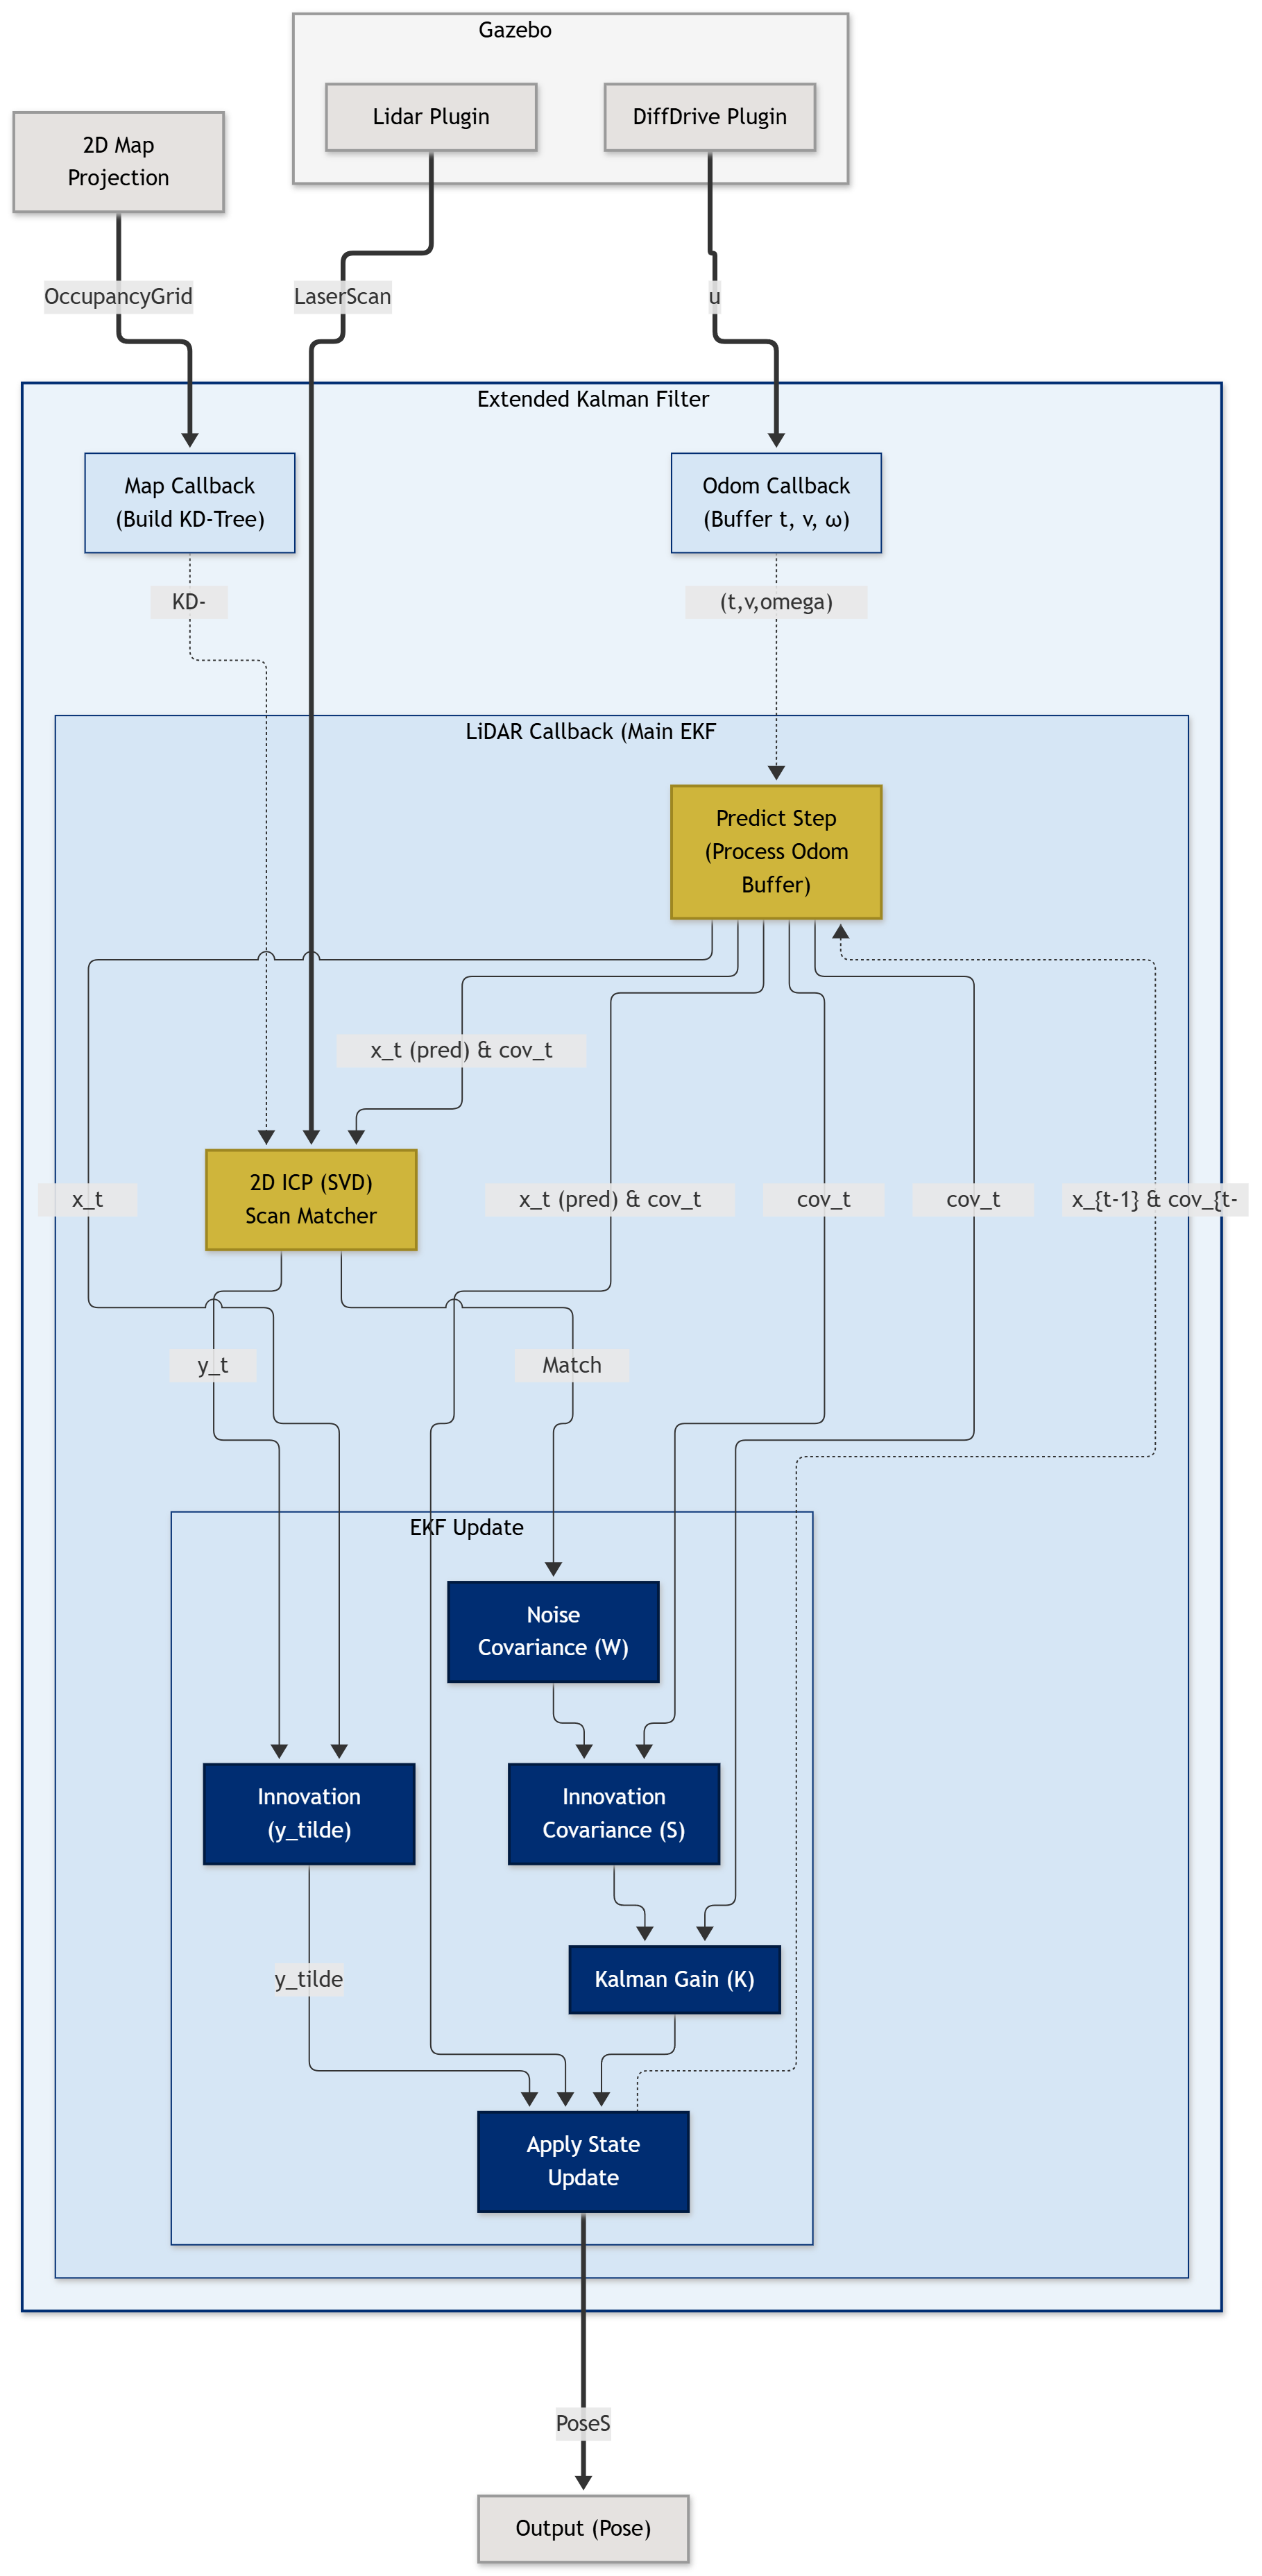
\includegraphics[width=0.65\textwidth]{figures/ekf.png}
    \caption{Extended Kalman Filter Update Algorithm}
    \label{fig:ekf}
\end{figure}

\subsubsection{Augmented Motion Model}\label{subsec:augmented-model}
During initial testing, there was a yaw-rate error that would build up in the EKF.
To mitigate this error, an augmented motion model was designed to include the state and the initial belief for the yaw-rate error which is shown in Equation \ref{eq:Augmented-State}.

\begin{equation}\label{eq:Augmented-State}
    \xi = \begin{bmatrix}
        x \\ y \\ \theta \\ s
    \end{bmatrix}
\end{equation}

The related covariance matrix is defined as $\textbf{P}\in\mathbb{R}^{4\times4}$ and the state and covariance are initialized as $\textbf{x}_0=[0,0,0,1]^T$ and $\textbf{P}_0=\text{diag}(0.1^2, 0.1^2, (5\pi/180)^2, 0.3^2)$.
Therefore the filter begins by assuming the odometry is unbiased ($\widehat{s}=1$), with a standard deviation of 0.3.

\textbf{Forward Kinematics} Substituting true yaw rate $s\omega$ for $\omega$ in Equation \ref{eq:discrete_unicycle_kinematics} and apending $s$.

\begin{equation}\label{eq:kinematics_augmented}
    f_a(\textbf{x},\textbf{u},\Delta t) = \bar{\textbf{x}}_t = \begin{bmatrix}
        x + v \cos(\theta) \Delta t \\ y + v \sin(\theta) \Delta t \\ \theta + s\omega \Delta t \\ s
    \end{bmatrix}
\end{equation}

\textbf{State Jacobian:} The state Jacobian $\textbf{A}_t$ is calculated by finding the partial derivatives of equation \ref{eq:discrete_unicycle_kinematics} with respect to $\textbf{x}$.

\begin{equation}\label{eq:state_jacobian_augmented}
    \textbf{A}_t = \frac{\partial \textbf{f}_a}{\partial \xi} = 
    \begin{bmatrix} 
        1 & 0 & -v \sin(\theta) \Delta t & 0 \\
        0 & 1 &  v \cos(\theta) \Delta t & 0 \\
        0 & 0 & 1                        & \omega \Delta t \\
        0 & 0 & 0                        & 1
    \end{bmatrix}
\end{equation}

\textbf{Control Jacobian:} The control Jacobian $\textbf{G}_t$ is calculated by finding the partial derivatives of equation \ref{eq:discrete_unicycle_kinematics} with respect to $\textbf{u}$.

\begin{equation}\label{eq:control_jacobian_augmented}
    \textbf{G}_t = \frac{\partial \textbf{f}_a}{\partial \textbf{u}} = 
    \begin{bmatrix} 
        \cos(\theta) \Delta t & 0  \\
        \sin(\theta) \Delta t & 0  \\
        0 & \Delta t \\
        0 & 0
    \end{bmatrix}
\end{equation}

\textbf{Process noise:} The process noise equation \ref{eq:mapped_process_noise} is then modified below to include a scaling factor for yaw $q_s$:

\begin{equation} \label{eq:mapped_process_noise_augmented}
    R_t = G_t M_t G_t^T \Delta t + \text{diag}(0,0,0,q_s^2 \Delta t)
\end{equation}

\subsubsection{Prediction}

The EKF prediction step is nearly identical to the Dead Reckoning process described in Section \ref{subsec:Dead-Reckoning:Prediction} except the Augmented Motion Model described in Section \ref{subsec:augmented-model} was used instead of the unicycle motion model.

\subsubsection{Measurement Update}
The observed pose $\textbf{z}_t$ and match error $\mathcal{M}$ come from Iterative Closest Point.
The observation matrix is the identify $H$.

\begin{equation}
    \textbf{H} = \begin{bmatrix}
        1 & 0 & 0 & 0 \\
        0 & 1 & 0 & 0 \\
        0 & 0 & 1 & 0
    \end{bmatrix}
\end{equation}

The innovation is found by Equation \ref{eq:ekf-innovation-cov}.

\begin{equation}\label{eq:ekf-innovation-cov}
    \tilde{y}_t = \textbf{z}_t - \hat{x}_t
\end{equation}

And the innovation covariance is found by Equation \ref{eq:ekf-innovation-cov}.

\begin{equation}\label{eq:ekf-innovation-cov}
    S_t = H \hat{\Sigma}_t H^T + W_t
\end{equation}

A $\chi^2$ statistical acceptance test is then performed to determine statistical acceptance using $\alpha=0.95$ and df$=3$.
If the observation is stastically reasonable, the Kalman gain $\textbf{K}$ is found by Equation \ref{eq:ekf-kalman-gain}

\begin{equation}\label{eq:ekf-kalman-gain}
    K = \hat{\Sigma} H^T S^{-1}
\end{equation}

Finally the state and covariances are updated as follows:
\begin{equation}\label{eq:ekf-state-update}
    \textbf{x}_t = \hat{x} + K \tilde{y}
\end{equation}

\begin{equation}\label{eq:ekf-cov-update}
    \Sigma_t = (I - K H) \hat{\Sigma}
\end{equation}

\textbf{Scan Matching via ICP and SVD:} 
The ICP algorithm implemented follows point-to-point descriptions from \textit{A Review of Point Cloud Registration Algorithms for Mobile Robotics} \cite{pomerleau2015review}.
It uses the predicted values $\bar{\textbf{x}_t}$ and $\bar{\Sigma_t}$, as well as, a KD-Tree built from the OccupancyGrid to output an observed state $\textbf{z}_t$ and a match error $\mathcal{M}$.
The \texttt{LaserScan} is processed into $\mathcal{P}$ and $\mathcal{Q}$ which represent the laser points in the localframe and the nearby collision points in the local frame, respectively.
First the centroid of the point clouds are found by:
\begin{equation}
    \mu_p = \frac{1}{K} \sum_{k = 1}^{K} p_k
\end{equation}

\begin{equation}
    \mu_q = \frac{1}{K} \sum_{k = 1}^{K} q_k
\end{equation}

The covariance is found as follows:

\begin{equation}
    \textbf{H} = \sum_{k = 1}^{K} (p_k - \mu_p) (q_k - \mu_q)^T
\end{equation}

Single Value Decomposition (SVD) is then used to find optimal transformation.
Let $\textbf{U}\varLambda \textbf{V}^T$ be the single value decomponsition $H$.
Then the optimal transformation to minimize the least squared error is shown in Equations \ref{eq:optimal-rotation} and \ref{eq:optimal-translation}:

\begin{equation}\label{eq:optimal-rotation}
    \widehat{R} = \textbf{V}\textbf{U}^T
\end{equation}

\begin{equation}\label{eq:optimal-translation}
    \widehat{t} = \mu_q - \widehat{R}\mu_p
\end{equation}

The observed pose $\textbf{z}_t$ is then found by applying the optimal transformation to $\bar{x}_t$.
The implementation of the EKF node and algorithm can be found in Appendix \ref{subsec:EKF implementation}.


\subsection{Particle Filter}

The Particle Filter, implemented as Monte Carlo Localization (MCL), represents the belief state using a set of weighted samples and evaluates the Bayes filter equations \ref{eq:bayes_prediction} and \ref{eq:bayes_measurement_update} by Monte Carlo simulation \cite{thrun2005probabilistic}.

\subsubsection{Prediction}
The Particle Filter begins the prediction step by creating noise proportional to the velocity commands for each particle using Equations \ref{eq:v-noise} and \ref{eq:omega-noise}.
It also includes a noise floor value $\sigma_{\omega,\min}=0.02$ to maintain particle spread while the robot is stationary.
Random noisy movements are then injected into the particles using a normal distribution.

\begin{equation}
    \Delta d^i \sim \mathcal{N}(v \Delta t, \sigma_v^2 \Delta t)
\end{equation}

\begin{equation}
    \Delta \varphi^i \sim \mathcal{N}(\omega \Delta t, \sigma_\omega^2 \Delta t)
\end{equation}

These values are then converted into per-particle velocities.

\begin{equation}
    v^i = \frac{\Delta d^i}{\Delta t}
\end{equation}

\begin{equation}
    \omega^i = \frac{\Delta \varphi^i}{\Delta t}
\end{equation}

These velocities are then applied to each particle using the forward kinematics described in Equation \ref{eq:discrete_unicycle_kinematics}.
An illustration of the PF prediction algorithm can be found in Figure \ref{fig:pf_prediction}.

\begin{figure}[!htbp]
    \centering
    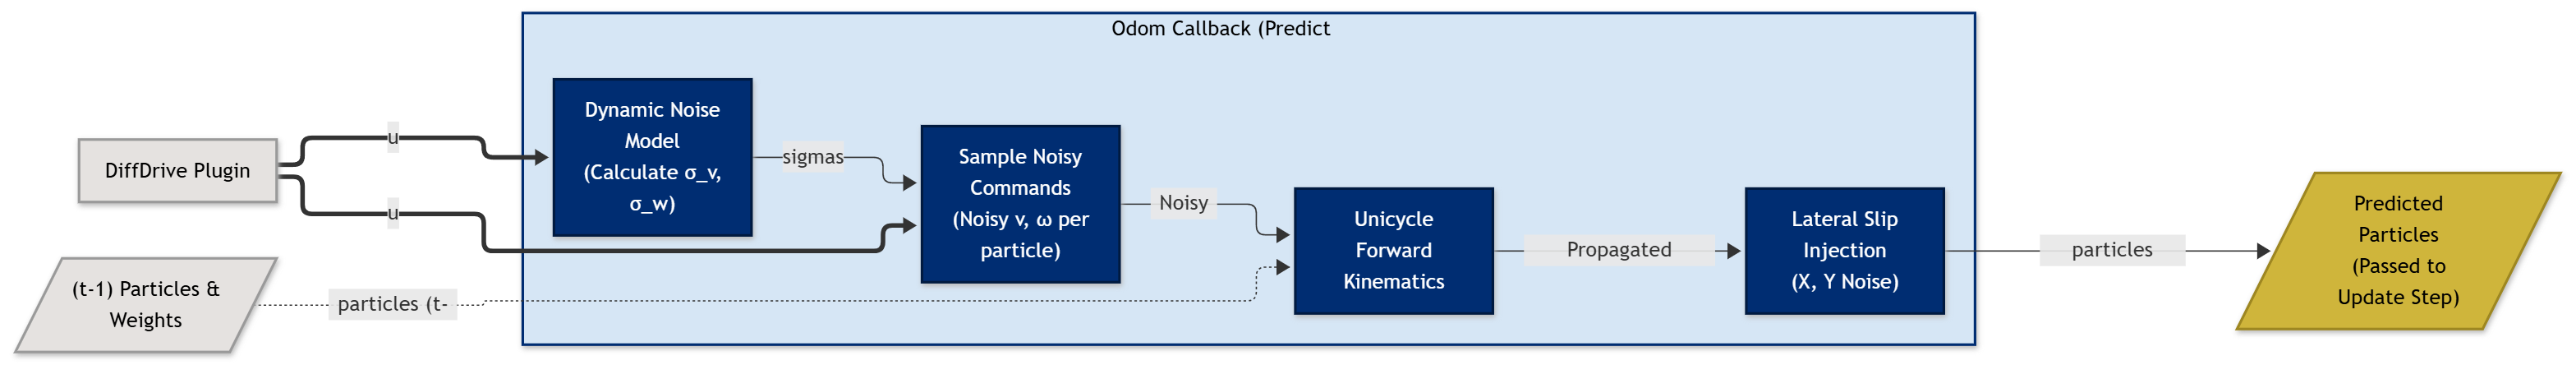
\includegraphics[width=\textwidth]{figures/pf_predict.png}
    \caption{Particle Filter Prediction Algorithm}
    \label{fig:pf_prediction}
\end{figure}

\subsubsection{Measurement Update}
The measurement step is illustrated in Figure \ref{fig:pf_update}.
The weight of each particle is updated using a Likelihood Field sensor model \cite{thrun2005probabilistic}. 
Rather than extracting a direct pose estimate from the scan like the EKF, the PF evaluates the raw LiDAR ranges against a pre-computed distance transform map found using SciPy \cite{scipyedt}. 
For a given particle pose hypothesis, each LiDAR endpoint $k$ is projected into the global map to find its Euclidean distance $d_k$ to the nearest obstacle. Assuming zero-mean Gaussian sensor noise with standard deviation $\sigma_{hit}$, the likelihood of a single beam is:
\begin{equation}
p(z_t^k \mid \mathbf{x}_t^{[m]}) \propto \exp \left( -\frac{d_k^2}{2\sigma_{hit}^2} \right)
\end{equation}
The total weight for particle $m$ is proportional to the product of the likelihoods of all valid beams. 
To prevent numerical underflow in floating-point operations, this is computed in log-space using the log-sum-exp trick:
\begin{equation}
w_t^{[m]} = \eta \exp \left( \sum_{k} \log p(z_t^k \mid \mathbf{x}_t^{[m]}) \right)
\end{equation}
where $\eta$ is a normalization constant ensuring that $\sum_{m=1}^M w_t^{[m]} = 1$.

\begin{figure}[!htbp]
    \centering
    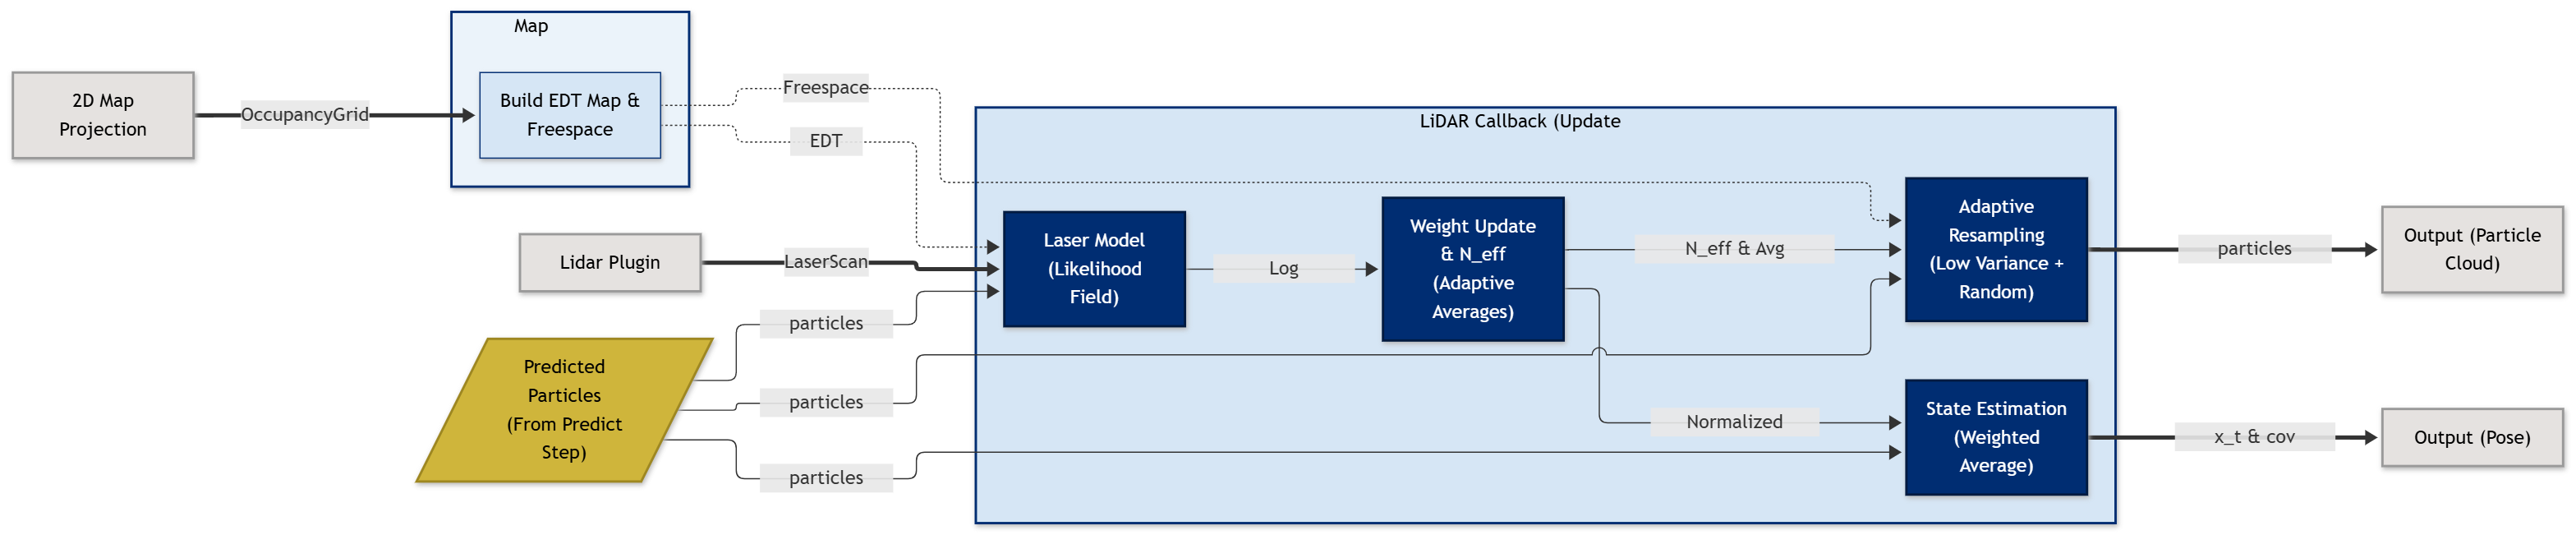
\includegraphics[width=\textwidth]{figures/pf_update.png}
    \caption{Particle Filter Update Algorithm}
    \label{fig:pf_update}
\end{figure}

\subsubsection{Resampling}
To prevent particle deprivation, where a majority of the computational effort is spent updating particles with near-zero weights, low-variance resampling is applied. 
A new set of $M$ particles is drawn from the current set with replacement, where the probability of drawing particle $m$ is proportional to its weight $w_t^{[m]}$. 
This focuses the distribution on the most probable regions of the state space.
The implementation of the PF node and algorithm can be found in Appendix \ref{subsec:PF implementation}.

\subsection{Kidnapping}
Kidnapping is performed by a seperate \texttt{Kidnap} node.
The Kidnap node monitors the ground truth state of the robot.
When the robot is within $0.3m$ of goal 1 pose, the Kidnap node starts a 15 second timer.
When the 15 second timer elaspes, the Kidnap node chooses a random valid position in free space and teleports the robot using a service call to Gazebo.
The local motion planner is robust to this and replans from its current pose to the existing goal (i.e. goal 2).

\subsection{Metric Collection}
Metric collection is performed by the \texttt{Metric} node.
The Metric node monitors the poses published by the localization nodes and compares them to the ground truth transform.
The Metric node compares the localization node poses with the ground truth pose to find the RMSE position and orientation values.
The Metric node also subscribes to the runtime topics for each localization nodes which includes runtime since their last estimation.
